\documentclass[11pt]{article}

\usepackage[a4paper, total={7in, 9.5in}]{geometry}
\usepackage{graphicx}
\usepackage{amssymb}
\usepackage{datetime}
\usepackage{pdfpages}
\usepackage{caption}
\usepackage{wrapfig}
\usepackage{tipa}
\usepackage{csvsimple}
\usepackage[T1]{fontenc}
\usepackage{hyperref}
\hypersetup{
	colorlinks=true,
	linkcolor=blue,
	filecolor=magenta,
	urlcolor=cyan,
	pdfpagemode=FullScreen,
}

\font\tenipa=tipa10
\def\schwa{{\tenipa\char64}}

\usepackage{array}
\newcolumntype{L}[1]{>{\raggedright\let\newline\\\arraybackslash\hspace{0pt}}p{#1}}
\newcolumntype{C}[1]{>{\centering\let\newline\\\arraybackslash\hspace{0pt}}p{#1}}
\newcolumntype{R}[1]{>{\raggedleft\let\newline\\\arraybackslash\hspace{0pt}}p{#1}}

\newdateformat{monthdayyeardate}{%
	\monthname[\THEMONTH]~\THEDAY, \THEYEAR}

\usepackage{setspace}
\usepackage{multirow}
\usepackage{xcolor}
\setlength{\parindent}{0em}
\setlength{\parskip}{0.5em}
\renewcommand{\baselinestretch}{1}

\begin{document}
\definecolor{myblue}{HTML}{3D4F7D}
\definecolor{myred}{HTML}{CD4F38}
\definecolor{mygreen}{HTML}{657060}
\definecolor{myorange}{HTML}{E48C2A}

\makebox[0pt][l]{%
  \raisebox{-\totalheight}[0pt][0pt]{%
  
\includegraphics{media/uvic.jpg}
  }}%


\hspace*{\fill}\textbf{Earth \& Ocean Sciences 240 A01}\\
% (CRN 21312)
\hspace*{\fill}\textbf{UNIVERSITY OF VICTORIA}\\
\hspace*{\fill}\textbf{3-3-0 (1.5 UNITS)}\\
\hspace*{\fill}\textbf{SPRING TERM 2025}\\


\noindent\hrulefill

\begin{center}
\emph{We acknowledge and respect the L\schwa\'k$^w$\schwa ŋ\schwa n (Songhees and Esquimalt) Peoples on whose territory the university stands, and the L\schwa\'k$^w$\schwa ŋ\schwa n and WS\'ANE\'C Peoples whose historical relationships with the land continue to this day.}
\end{center}

\noindent\hrulefill

\begin{center}
\Large \textbf{COURSE OUTLINE}

\Large \textbf{EOS240: Geochemistry}

\normalsize Lectures: M/Th 10:00 to 11:20 AM in Cornett B108  \\
\end{center}

\noindent\hrulefill

\textbf{PREREQUISITES}: EOS110, EOS120, EOS205, 1 of CHEM254, PHYS217, PHYS317\\
\textbf{COREQUISITES}: NONE\\

\textbf{CONTACT INFO}

\begin{center}
  \centering
  \begin{tabular}{ L{.25\linewidth}L{.25\linewidth}L{.25\linewidth} }
    Instructor(s):      & Blake Dyer &  \\
    Email:      & blakedyer@uvic.ca &  \\
    Office:      & BWC A419 &  \\
    Office Hours:      & M 3:00 to 4:00 PM &  \\
          &  &  \\
    Lab Coordinator      & Eva MacLennan &  evamegan@uvic.ca\\
Teaching Assistant(s)      & XXXX & XXXX@xxxx.com \\
      & XXXX & XXXX@xxxx.com \\
  \end{tabular}\\
\end{center}

\begin{center}
\textbf{COURSE DESCRIPTION}
\end{center}

In geochemistry, we use the tools of chemistry to understand the Earth and how it works. Principles of thermodynamics and kinetics will be applied to understand key processes that control of the geochemistry of the Earth, from the low temperature and pressure conditions of Earth's surface environment to higher temperature and pressure conditions in Earth's interior. We will consider processes operating on time scales of millions (planetary formation) to hundreds (climate change) of years. The lab will provide hands-on experience using real data to solve geological problems.

% KEY THEMES: [keywords]

\clearpage

\textbf{LEARNING OUTCOMES}

Below is a list of some specific knowledge and skills you can expect to gain through this course. This term you will:
\begin{itemize}
	\setlength\itemsep{0em}
\csvreader[	head to column names, 
			before reading={\catcode`\"=9},
  			after reading={\catcode`\"=13}]
        {tables/learning_outcomes.csv}{1=\learningoutcome}
        {\item \learningoutcome}
\end{itemize}

\textbf{COURSE MATERIALS}

There is no required textbook. Students are required to have access to a computer to work on assignments. Please let us know if you do not have access to a computer. Lab material and supplemental readings will be made available through the course Brightspace page.


\textbf{BRIGHTSPACE}

You are expected to routinely check the Brightspace site. All announcements, materials, supplemental readings, and schedule changes will be posted to brightspace.


\begin{center}
  \textbf{EVALUATION}
\end{center}

This course will use the \href{https://www.uvic.ca/calendar/future/undergrad/index.php#/policy/S1AAgoGuV?bc=true&bcCurrent=14%20-%20Grading&bcGroup=Undergraduate%20Academic%20Regulations&bcItemType=policies}{official UVic standard grading scale}. Your final grade will be determined by your scores on in-class exams and weekly laboratory assignments. Lab assignments \textbf{will require additional time} beyond the scheduled three hour lab period. These assignments are due before the next lab meeting (1 week to complete). There is no final exam.

\begin{center}
		\begin{tabular}{ lr }
			Lecture                     & 50\%       \\
			\hline
			~~~Mid-term (Feb 13, week 6)  & 25\%~~~~~~ \\
			~~~Final Exam (date TBA) & 25\%~~~~~~ \\
			Laboratory                  & 50\%       \\
			\hline
			~~~9 Lab Assignments    & 50\%~~~~~~  \\
		\end{tabular}
\end{center}

\textbf{Students must pass ($>50\%$) both the lab and lecture portion of this course to pass the course. In other words, a 100\% average on the labs and a 49\% average on the in class exams will result in a failing final grade (and vice versa).}

\begin{center}
  \textbf{COURSE POLICIES}
\end{center}

If you need academic accommodation to address barriers to your education, please register with the Centre for Accessible Learning (CAL) as soon as possible. We work with the CAL to create a learning environment that is equitable, inclusive, and usable for all.

\textbf{POLICY: CLASS CONDUCT}

Please follow the latest provincial and University guidelines with regard to COVID-19 protocols: \href{https://www.uvic.ca/covid19/index.php}{UVic COVID-19 information} and \href{https://www.uvic.ca/covid19/health-safety/index.php#ipn-if-you-re-sick}{what to do if you are ill}. No materials from the course may be redistributed without written permission from the instructors (e.g., no posting of materials to sharing websites). If we are required to meet on Zoom, you should remain muted during lecture unless you are speaking to the class or instructors.

\textbf{POLICY: LATE/MISSED ASSIGNMENTS OR EXAMINATIONS}

Students are required to complete all exams to recieve a final grade in the course. If you must miss the an exam for a valid reason (illness, accident, family emergency etc.), you must notify the instructor as soon as possible, and you may be asked to provide documentation to support your request. If you miss an exam \textbf{with a valid excuse}, we will arrange a make up exam.

If a student does not sit an exam, they will be assigned a grade of \textbf{N} regardless of their performance in other elements of the course. A grade of \textbf{N} is a failing grade and will be scored as a zero in the calculation of the students CGPA. The maximum percentage grade that can be assigned for a student achieving a \textbf{N} grade is 49\%. 

The general approach to late submissions of lab assignments is a 10\% grade penalty per day. Late assignments will not be accepted after marked assignments have been returned to others. However, if you know that you will miss a deadline due to a personal emergency, please let your lab instructors know as soon as possible and we will do our best to work with you to find a solution.

\textbf{POLICY: ATTENDANCE}

You are expected to be present and active in the lectures. We will not formally track participation in lecture, but from past experience we know that the assignments will be significantly easier to complete and exam scores are higher for those who attend and participate in lecture. Laboratory attendance is mandatory. If you will miss a lab for medical or other valid reasons, please contact the Lab Coordinator as soon as possible. Recall that \textbf{you must pass the lab to pass the course}.

\textbf{POLICY: ACADEMIC INTEGRITY}

It is every student's responsibility to be aware of the university's \href{https://web.uvic.ca/calendar/undergrad/info/regulations/academic-integrity.html}{policies on ccademic integrity}, including policies on cheating, plagiarism, unauthorized use of an editor, multiple submission, and aiding others to cheat. 

If you have any questions or doubts, you can ask your course instructor or the \href{https://uvic.ca/learningandteaching/cac}{Centre for Academic Communication}.

\begin{center}
  \textbf{COURSE FEEDBACK}
\end{center}

I value your feedback on this course. Towards the end of term, as in all other courses at UVic, you will have the opportunity to complete an anonymous survey regarding your learning experience (CES). \textbf{The survey is vital for providing feedback} to me regarding the course and my teaching, as well as to help the department improve the overall program for students in the future. The survey is accessed online and can be done on your laptop, tablet, or mobile device. I will remind you and provide you with more detailed information nearer the time but please be thinking about this important activity during the course.

\begin{minipage}{\textwidth}

\begin{center}
  \textbf{COURSE WEEKLY CALENDAR}
\end{center}

This calendar will get updated throughout the term (last updated on: {\color{myred}\monthdayyeardate\today}). Exam dates are set, but lecture and lab topics are subject to change. 

\begin{tabular}{C{.06\linewidth}R{.12\linewidth}L{.76\linewidth}}
  \bfseries Week & \bfseries Date & \bfseries \hfill Lecture Topic\\
\csvreader[no head,late after line = \\]
        {tables/schedule.csv}{1=\wk,2=\dy,3=\mn,4=\daten,5=\subtcolor,6=\subt,7=\ltopic,8=\readings}
        {\bfseries \wk & \bfseries \dy~\mn~\daten & {\color{\subtcolor}\textbf{\subt}}\dotfill{\color{\subtcolor}\textbf{\ltopic}}}
\end{tabular}

\end{minipage}

\clearpage

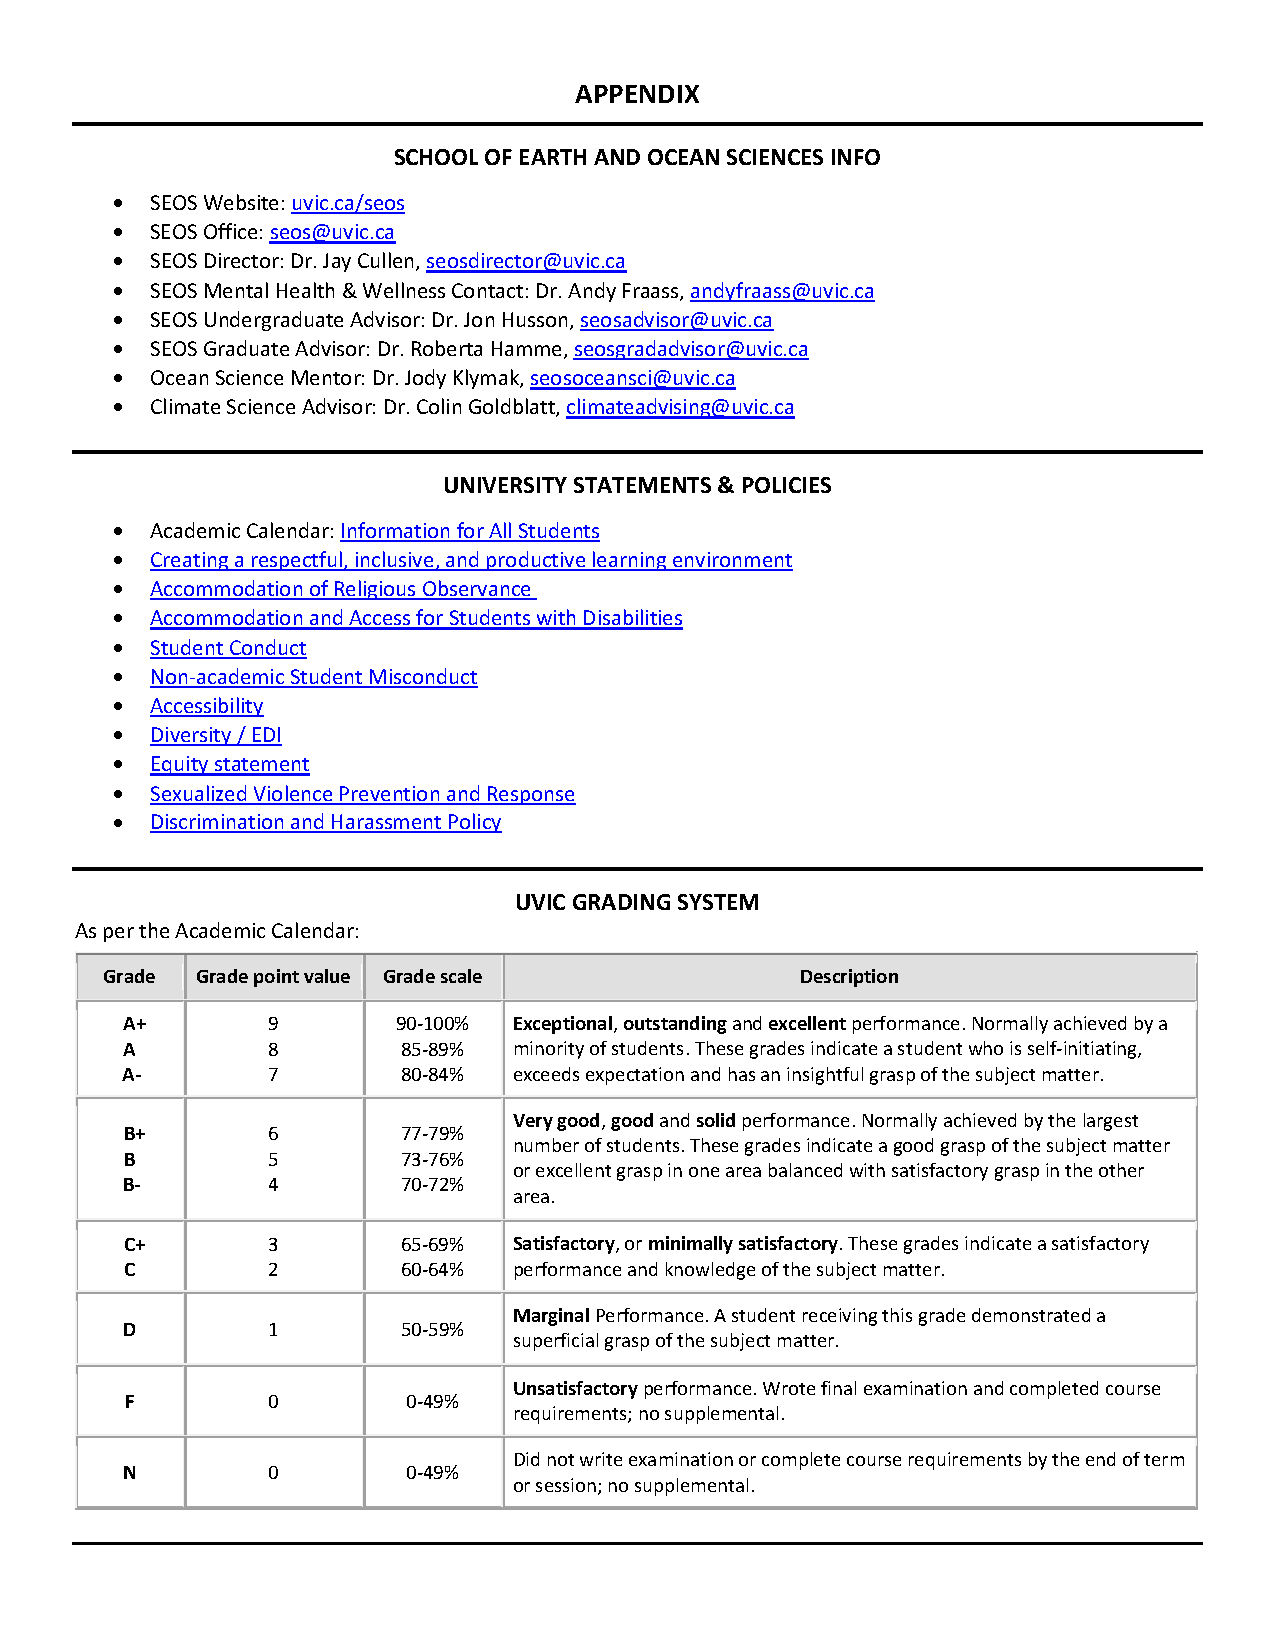
\includepdf[pages=-,pagecommand={},width=\textwidth]{Appendix.pdf}

\end{document}
